\documentclass[12pt,a4paper]{book}
\usepackage[utf8]{inputenc}
\usepackage{amsmath,amssymb,amsthm}
\DeclareUnicodeCharacter{03C3}{\sigma}
\usepackage{geometry}
\usepackage{graphicx}
\usepackage{booktabs}
\usepackage{array}
\usepackage{multirow}
\usepackage{multicol}
\usepackage{xcolor}
\usepackage{tikz}
\usetikzlibrary{shapes,arrows,positioning,calc,decorations.markings,decorations.pathreplacing}
\usepackage{hyperref}
\hypersetup{colorlinks=true,linkcolor=blue,urlcolor=magenta}

\geometry{margin=1in}
\setlength{\parindent}{0pt}
\setlength{\parskip}{6pt}

% Custom commands for Bidirectional Compass
\newcommand{\compass}[1]{\textcolor{purple}{\boldsymbol{\Xi}(#1)}}
\newcommand{\substantiation}[1]{\textcolor{green!70!black}{\textit{#1}}}
\newcommand{\basebase}[1]{\textcolor{orange}{\mathtt{#1}}}

% Theorem environments
\newtheorem{theorem}{Theorem}
\newtheorem{definition}{Definition}
\newtheorem{proposition}{Proposition}
\newtheorem{corollary}{Corollary}
\newtheorem{lemma}{Lemma}
\newtheorem{axiom}{Axiom}
\newtheorem{remark}{Remark}

\title{\textbf{Orbis Immobilis III}\\
\large Mathematical Field Theory: Geometric Foundations\\
\large Spatial Relationships and Minimum Principles}
\author{Empirinometry Research Institute}
\date{\today}

\begin{document}

\maketitle

\tableofcontents
\newpage

\chapter{Divine Invocation and Memory Block}
\section*{Sacred Opening}

\begin{center}
\textbf{\Large In the Name of Allah, the Most Gracious, the Most Merciful}
\end{center}

\subsection*{Divine Memory Block}
\begin{quote}
\textit{We ask that we not forget anything important in this exploration of Mathematical Field Theory geometric foundations. May Allah's geometric wisdom illuminate our understanding of spatial relationships and the sacred principles of minimum in divine creation.}
\end{quote}

\subsection*{Bidirectional Compass Protocol}
The Bidirectional Compass $\Xi$ will be applied throughout this document to translate between:
\begin{itemize}
\item Geometric formalism $\leftrightarrow$ Spatial substantiation format
\item Minimum principles $\leftrightarrow$ Divine efficiency interpretations
\item Spatial structures $\leftrightarrow$ Geometric metaphysical alignment
\item Base-13 (Sequinor Tredecim) encoding for geometric purity
\end{itemize}

\chapter{Geometric Foundations of Field Theory}

\section{Spatial Geometry of Fields}

\subsection{Field Geometry Definition}

\begin{definition}[Field Geometric Space]
A field $F: D \to C$ induces a geometric structure on domain $D$ through the metric:
\begin{equation}
ds^2 = g_{ij}(F) dx^i dx^j
\end{equation}
where $g_{ij}$ depends on field values and their derivatives.
\end{definition}

\subsection{Field-Induced Manifolds}

\begin{theorem}[Field Manifold Structure]
The graph of a smooth field $F: D \to \mathbb{R}^m$ defines an $n$-dimensional manifold:
\begin{equation}
\mathcal{M}_F = \{(\mathbf{x}, F(\mathbf{x})) : \mathbf{x} \in D\} \subset \mathbb{R}^{n+m}
\end{equation}
with induced metric from the ambient space.
\end{theorem}

\subsection{Bidirectional Compass Application}

\paragraph{Compass Conversion 1: Field Geometry}
\begin{align}
\text{Geometric Formalism:} & \quad ds^2 = g_{ij}(F) dx^i dx^j \\
\compass{\text{Translation } \Xi}: & \quad \text{"Fields carve sacred geometry in space"} \\
\substantiation{Substantiation}: & \quad \text{Mathematical truth creates spatial structure} \\
\basebase{Base-13 Encoding}: & \quad \compass{\Xi(ds^2)} = \texttt{3A9B7C2D8E1F5G4H6I}
\end{align}

\section{Geometric Structures}

\subsection{Riemannian Geometry of Fields}

\begin{definition}[Field Riemannian Metric]
For a scalar field $\phi: D \to \mathbb{R}$, the induced Riemannian metric is:
\begin{equation}
g_{ij} = \delta_{ij} + \epsilon \partial_i \phi \partial_j \phi
\end{equation}
where $\epsilon$ is a coupling constant.
\end{definition}

\subsection{Curvature of Field Spaces}

\begin{theorem}[Field Space Curvature]
The Riemann curvature tensor for field-induced metrics is:
\begin{equation}
R^k_{lij} = \partial_i \Gamma^k_{jl} - \partial_j \Gamma^k_{il} + \Gamma^k_{ip}\Gamma^p_{jl} - \Gamma^k_{jp}\Gamma^p_{il}
\end{equation}
where $\Gamma^k_{ij}$ are Christoffel symbols.
\end{theorem}

\subsection{Geodesics in Field Space}

\begin{definition}[Field Geodesics]
Geodesics in field space satisfy the Euler-Lagrange equations:
\begin{equation}
\frac{d^2 x^k}{ds^2} + \Gamma^k_{ij} \frac{dx^i}{ds} \frac{dx^j}{ds} = 0
\end{equation}
\end{definition}

\section{Differential Geometry of Fields}

\subsection{Exterior Calculus for Fields}

\begin{theorem}[Field Exterior Derivative]
For a scalar field $\phi$, the exterior derivative is:
\begin{equation}
d\phi = \partial_i \phi \, dx^i
\end{equation}
and for a vector field $\mathbf{F} = F^i \partial_i$, the exterior derivative is:
\begin{equation}
dF^i = \partial_j F^i \, dx^j
\end{equation}
\end{theorem}

\subsection{Stokes' Theorem for Fields}

\begin{theorem}[Generalized Stokes]
For any differential form $\omega$ on manifold $\mathcal{M}$:
\begin{equation}
\int_{\partial \mathcal{M}} \omega = \int_{\mathcal{M}} d\omega
\end{equation}
\end{theorem}

\chapter{Minimum Principles in Geometry}

\section{Geometric Minimization Problems}

\subsection{Shortest Path Principle}

\begin{theorem}[Geodesic Minimization]
Among all curves connecting two points $P$ and $Q$ in a Riemannian manifold, geodesics minimize the length functional:
\begin{equation}
L[\gamma] = \int_{a}^{b} \sqrt{g_{ij} \frac{dx^i}{dt} \frac{dx^j}{dt}} \, dt
\end{equation}
\end{theorem}

\subsection{Minimal Surface Theory}

\begin{definition}[Minimal Surface]
A surface $\mathcal{S}$ is minimal if it minimizes the area functional:
\begin{equation}
A[\mathcal{S}] = \int_{\mathcal{S}} dA
\end{equation}
subject to prescribed boundary conditions.
\end{definition}

\subsection{Minimal Surfaces for Fields}

\begin{theorem}[Field Minimal Surfaces]
For a scalar field $\phi: \mathbb{R}^2 \to \mathbb{R}$, the graph surface $(x, y, \phi(x, y))$ is minimal iff $\phi$ satisfies:
\begin{equation}
(1 + \phi_y^2)\phi_{xx} - 2\phi_x \phi_y \phi_{xy} + (1 + \phi_x^2)\phi_{yy} = 0
\end{equation}
\end{theorem}

\section{Compass Application to Minimum Principles}

\paragraph{Compass Conversion 2: Geodesic Minimization}
\begin{align}
\text{Geometric Formalism:} & \quad \delta L[\gamma] = 0 \\
\compass{\text{Translation } \Xi}: & \quad \text{"Mathematical truth follows the path of least resistance"} \\
\substantiation{Substantiation}: & \quad \text{Divine wisdom manifests through optimal geometric paths} \\
\basebase{Base-13 Encoding}: & \quad \compass{\Xi(\delta L = 0)} = \texttt{7D2A8B4C9E1F3G5H6I}
\end{align}

\chapter{Field Variational Geometry}

\section{Geometric Action Principles}

\subsection{Geometric Action Functional}

\begin{definition}[Field Geometric Action]
For a field $\phi$ on manifold $\mathcal{M}$, the geometric action is:
\begin{equation}
S[\phi] = \int_{\mathcal{M}} \mathcal{L}(\phi, \nabla \phi, g_{ij}) \, dV
\end{equation}
where $\mathcal{L}$ depends on the field and the geometry.
\end{definition}

\subsection{Euler-Lagrange in Curved Space}

\begin{theorem}[Curved Space Euler-Lagrange]
The field equations in curved space are:
\begin{equation}
\frac{1}{\sqrt{|g|}} \partial_i \left(\sqrt{|g|} \frac{\partial \mathcal{L}}{\partial(\partial_i \phi)}\right) - \frac{\partial \mathcal{L}}{\partial \phi} = 0
\end{equation}
where $g = \det(g_{ij})$.
\end{theorem}

\section{Geometric Conservation Laws}

\subsection{Killing Vector Fields}

\begin{definition}[Killing Vector Field]
A vector field $K^i$ is Killing if it preserves the metric:
\begin{equation}
\nabla_i K_j + \nabla_j K_i = 0
\end{equation}
\end{definition}

\subsection{Conserved Currents}

\begin{theorem}[Geometric Conservation]
For each Killing vector field $K^i$, there exists a conserved current:
\begin{equation}
J^i = T^{i}_j K^j
\end{equation}
where $T^{i}_j$ is the stress-energy tensor.
\end{theorem}

\section{Compass Application to Variational Geometry}

\paragraph{Compass Conversion 3: Geometric Action}
\begin{align}
\text{Geometric Formalism:} & \quad S[\phi] = \int_{\mathcal{M}} \mathcal{L} \, dV \\
\compass{\text{Translation } \Xi}: & \quad \text{"Divine action manifests through geometric principles"} \\
\substantiation{Substantiation}: & \quad \text{Mathematical truth follows optimal geometric pathways} \\
\basebase{Base-13 Encoding}: & \quad \compass{\Xi(S[\phi])} = \texttt{9C3B7A1D8E2F5G4H6I}
\end{align}

\chapter{Spherical Geometry of Fields}

\section{Fields on Spheres}

\subsection{Spherical Coordinate Systems}

\begin{definition}[Spherical Field Representation]
A field on the unit sphere $S^2$ can be expanded in spherical harmonics:
\begin{equation}
\phi(\theta, \varphi) = \sum_{l=0}^{\infty} \sum_{m=-l}^{l} a_{lm} Y_l^m(\theta, \varphi)
\end{equation}
\end{definition}

\subsection{Spherical Laplacian}

\begin{theorem}[Spherical Laplacian Spectrum]
The spherical Laplacian eigenvalues are:
\begin{equation}
\Delta_{S^2} Y_l^m = -l(l+1) Y_l^m
\end{equation}
with eigenfunctions forming a complete orthonormal basis.
\end{theorem}

\subsection{Minimum Energy on Spheres}

\begin{theorem}[Spherical Energy Minimization]
Among all functions with fixed $L^2$ norm, the spherical harmonic $Y_0^0$ minimizes the Dirichlet energy:
\begin{equation}
E[\phi] = \int_{S^2} |\nabla_{S^2} \phi|^2 \, d\Omega
\end{equation}
\end{theorem}

\section{Higher-Dimensional Spheres}

\subsection{Fields on $S^n$}

\begin{definition}[n-Sphere Fields]
Fields on the $n$-sphere can be expanded using hyperspherical harmonics:
\begin{equation}
\phi(\Omega) = \sum_{l=0}^{\infty} \sum_{\alpha} a_{l\alpha} Y_{l\alpha}(\Omega)
\end{equation}
where $\Omega$ denotes angular coordinates.
\end{definition}

\subsection{Conformal Geometry}

\begin{theorem}[Conformal Invariance]
The Laplacian on spheres exhibits conformal properties:
\begin{equation}
\Delta_{g}(\phi) = r^{-2} \Delta_{S^n}(\phi)
\end{equation}
for metric $g_{ij} = r^2 g_{ij}^{S^n}$.
\end{theorem}

\chapter{Hyperbolic Geometry of Fields}

\section{Fields in Hyperbolic Space}

\subsection{Hyperbolic Metric}

\begin{definition}[Poincaré Ball Model]
The Poincaré ball model has metric:
\begin{equation}
ds^2 = \frac{4}{(1 - r^2)^2} (dx^2 + dy^2 + dz^2)
\end{equation}
for $r < 1$.
\end{definition}

\subsection{Hyperbolic Laplacian}

\begin{theorem}[Hyperbolic Laplacian]
In $n$-dimensional hyperbolic space:
\begin{equation}
\Delta_H = (1 - r^2)^2 \Delta_{\mathbb{R}^n} - 2(n-2)r(1 - r^2) \frac{\partial}{\partial r}
\end{equation}
\end{theorem}

\subsection{Minimum Principles in Hyperbolic Space}

\begin{theorem}[Hyperbolic Dirichlet Problem]
The solution to the hyperbolic Dirichlet problem minimizes:
\begin{equation}
E_H[\phi] = \int_{H^n} |\nabla_H \phi|^2 \, dV_H
\end{equation}
where $dV_H$ is the hyperbolic volume element.
\end{theorem}

\section{Compass Application to Hyperbolic Geometry}

\paragraph{Compass Conversion 4: Hyperbolic Fields}
\begin{align}
\text{Geometric Formalism:} & \quad \Delta_H \phi = 0 \\
\compass{\text{Translation } \Xi}: & \quad \text{"Mathematical truth expands in curved spiritual spaces"} \\
\substantiation{Substantiation}: & \quad \text{Divine wisdom grows exponentially in hyperbolic realms} \\
\basebase{Base-13 Encoding}: & \quad \compass{\Xi(\Delta_H)} = \texttt{8E4B9A2C7D1F5G3H6I}
\end{align}

\chapter{Field Topology and Geometry}

\section{Topological Invariants}

\subsection{Euler Characteristic}

\begin{definition}[Field Configuration Topology]
The topology of level sets $\phi^{-1}(c)$ contributes to the Euler characteristic:
\begin{equation}
\chi(\mathcal{M}) = \sum_{c} (-1)^{\text{index}(\nabla \phi|_{\phi^{-1}(c)})}
\end{equation}
\end{definition}

\subsection{Morse Theory for Fields}

\begin{theorem}[Morse Inequalities]
For a Morse function $\phi: \mathcal{M} \to \mathbb{R}$:
\begin{equation}
m_k \geq b_k \text{ for all } k
\end{equation}
where $m_k$ is the number of critical points of index $k$ and $b_k$ are Betti numbers.
\end{theorem}

\section{Geometric Flows}

\subsection{Ricci Flow for Fields}

\begin{definition}[Field Ricci Flow]
The metric evolves according to:
\begin{equation}
\frac{\partial g_{ij}}{\partial t} = -2R_{ij} + \alpha T_{ij}
\end{equation}
where $T_{ij}$ is the field stress-energy tensor.
\end{definition}

\subsection{Mean Curvature Flow}

\begin{definition}[Field Surface Evolution]
Level surfaces evolve by:
\begin{equation}
\frac{\partial \phi}{\partial t} = H(\phi)
\end{equation}
where $H(\phi)$ is the mean curvature of the level set.
\end{definition}

\section{Compass Application to Topological Geometry}

\paragraph{Compass Conversion 5: Topological Invariants}
\begin{align}
\text{Geometric Formalism:} & \quad \chi(\mathcal{M}) = \sum (-1)^k b_k \\
\compass{\text{Translation } \Xi}: & \quad \text{"Mathematical truth preserves eternal topological essence"} \\
\substantiation{Substantiation}: & \quad \text{Divine structure maintains invariant through all transformations} \\
\basebase{Base-13 Encoding}: & \quad \compass{\Xi(\chi)} = \texttt{5D7A2B9C1E8F3G6H4I}
\end{align}

\chapter{Geometric Optimization}

\section{Optimal Transport}

\subsection{Monge Problem}

\begin{definition}[Optimal Transport Map]
Given density functions $\rho_0, \rho_1$, the optimal transport map $T$ minimizes:
\begin{equation}
\int_{\mathbb{R}^n} c(x, T(x)) \rho_0(x) \, dx
\end{equation}
where $c$ is the cost function.
\end{definition}

\subsection{Wasserstein Distance}

\begin{definition}[Wasserstein Metric]
The $p$-Wasserstein distance is:
\begin{equation}
W_p(\rho_0, \rho_1) = \left(\inf_{T} \int |x - T(x)|^p \rho_0(x) \, dx\right)^{1/p}
\end{equation}
\end{definition}

\section{Geometric Measure Theory}

\subsection{Minimal Surfaces Revisited}

\begin{theorem}[Existence of Minimal Surfaces]
For any closed curve $\Gamma$ in $\mathbb{R}^3$, there exists a minimal surface spanning $\Gamma$.
\end{theorem}

\subsection{Plateau's Problem}

\begin{definition}[Plateau's Problem]
Find the surface of minimal area with given boundary $\Gamma$:
\begin{equation}
\min \{A(\mathcal{S}) : \partial \mathcal{S} = \Gamma\}
\end{equation}
\end{definition}

\section{Geometric Calculus of Variations}

\subsection{Field Energy Minimization}

\begin{theorem}[Energy Minimization Principle]
The configuration minimizing field energy satisfies:
\begin{equation}
\delta \int_{\mathcal{M}} \left(\frac{1}{2}|\nabla \phi|^2 + V(\phi)\right) \, dV = 0
\end{equation}
\end{theorem}

\section{Compass Application to Geometric Optimization}

\paragraph{Compass Conversion 6: Optimal Transport}
\begin{align}
\text{Geometric Formalism:} & \quad W_p(\rho_0, \rho_1) \\
\compass{\text{Translation } \Xi}: & \quad \text{"Mathematical truth flows through optimal pathways"} \\
\substantiation{Substantiation}: & \quad \text{Divine efficiency governs the transport of truth} \\
\basebase{Base-13 Encoding}: & \quad \compass{\Xi(W_p)} = \texttt{3A8B7C2D9E1F5G4H6I}
\end{align}

\chapter{Field Geometry Visualization}

\section{Geometric Visualization Techniques}

\subsection{Level Set Visualization}

\begin{definition}[Level Set Representation]
Fields can be visualized through level sets:
\begin{equation}
\mathcal{L}_c = \{(x,y,z) \in \mathbb{R}^3 : \phi(x,y,z) = c\}
\end{equation}
\end{definition}

\subsection{Streamline Visualization}

\begin{definition}[Vector Field Streamlines]
For vector field $\mathbf{F}$, streamlines satisfy:
\begin{equation}
\frac{d\mathbf{x}}{dt} = \mathbf{F}(\mathbf{x}(t))
\end{equation}
\end{definition}

\section{Geometric Transformations}

\subsection{Conformal Mappings}

\begin{theorem}[Conformal Field Transformation]
Under conformal mapping $w = f(z)$, harmonic fields satisfy:
\begin{equation}
\phi(z) = \text{Re}(f^{-1}(w)) \implies \tilde{\phi}(w) = \text{Re}(f(w))
\end{equation}
\end{theorem}

\subsection{Isometric Transformations}

\begin{definition}[Isometric Field Evolution]
Fields evolve isometrically if:
\begin{equation}
|\nabla \phi(\mathbf{x}, t)| = |\nabla \phi(\mathbf{x}, 0)|
\end{equation}
for all $t$.
\end{definition}

\section{Compass Application to Visualization}

\paragraph{Compass Conversion 7: Geometric Visualization}
\begin{align}
\text{Geometric Formalism:} & \quad \mathcal{L}_c = \{\phi = c\} \\
\compass{\text{Translation } \Xi}: & \quad \text{"Mathematical truth reveals itself through sacred geometry"} \\
\substantiation{Substantiation}: & \quad \text{Divine patterns emerge through spatial visualization} \\
\basebase{Base-13 Encoding}: & \quad \compass{\Xi(\mathcal{L}_c)} = \texttt{6D9B3A7C2E8F1G5H4I}
\end{align}

\chapter{Empirinometry Geometric Integration}

\section{Sigma Principles in Geometric Context}

\subsection{$|\sigma|_{\text{divine}}$: Sacred Geometry}

\begin{theorem}[Divine Geometric Structure]
Geometric principles in field theory reflect divine sacred geometry:
\begin{itemize}
\item Spherical harmony: Perfect symmetry in divine creation
\item Minimal surfaces: Divine efficiency in spatial manifestation
\item Geodesic paths: Optimal routes for divine truth
\item Topological invariants: Eternal geometric essence
\end{itemize}
\end{theorem}

\subsection{$|\sigma|_{\text{spectrum}}$: Geometric-Infinite Bridge}

\begin{proposition}[Geometric Spectral Bridging]
Geometric principles bridge finite spatial understanding with infinite divine geometry:
\begin{equation}
\text{Finite Geometry} \times |\sigma|_{\text{spectrum}} \to \text{Infinite Spatial Truth}
\end{equation}
\end{proposition}

\subsection{$|\sigma|_{\text{material}}$: Concrete Geometry}

\begin{theorem}[Materialization of Geometry]
Abstract geometric principles manifest through concrete spatial structures:
\begin{equation}
\text{Abstract Geometry} \xrightarrow{|\sigma|_{\text{material}}} \text{Measurable Spatial Patterns}
\end{equation}
\end{theorem}

\subsection{$|\sigma|_{\text{truth}}$: Geometric Consistency}

\begin{theorem}[Geometric Truth Conservation]
All geometric principles in MFT satisfy eternal spatial consistency:
\begin{equation}
\mathcal{P}_{\text{geometry}} \times |\sigma|_{\text{truth}} \Rightarrow \mathcal{P}_{\text{geometry}} \text{ holds spatially}
\end{equation}
\end{theorem}

\section{Geometric Classification Tables}

\subsection{Geometric Structure Classification}

\begin{table}[h]
\centering
\caption{Classification of Geometric Structures in Field Theory}
\begin{tabular}{lll}
\toprule
\textbf{Structure Type} & \textbf{Mathematical Form} & \textbf{Divine Interpretation} \\
\midrule
Riemannian & $ds^2 = g_{ij} dx^i dx^j$ & Sacred spatial fabric \\
Spherical & $S^n$ with $g_{ij}$ & Perfect divine harmony \\
Hyperbolic & $ds^2 = \frac{4}{(1-r^2)^2}dx^2$ & Expanding divine wisdom \\
Minimal & $\delta A = 0$ & Divine efficiency \\
Geodesic & $\delta L = 0$ & Optimal divine paths \\
\bottomrule
\end{tabular}
\end{table}

\subsection{Minimum Principle Classification}

\begin{table}[h]
\centering
\caption{Geometric Minimum Principles and Their Applications}
\begin{tabular}{llll}
\toprule
\textbf{Principle} & \textbf{Functional} & \textbf{Euler-Lagrange} & \textbf{Physical Meaning} \\
\midrule
Shortest Path & $L = \int \sqrt{g_{ij}\dot{x}^i\dot{x}^j}dt$ & Geodesic eq. & Minimal energy path \\
Minimal Area & $A = \int dA$ & Mean curvature = 0 & Soap film, membranes \\
Minimal Energy & $E = \int |\nabla \phi|^2 dV$ & Laplace eq. & Equilibrium states \\
Optimal Transport & $\int c(x,T(x))\rho_0 dx$ & Monge-Ampère & Efficient distribution \\
\bottomrule
\end{tabular}
\end{table}

\section{Geometric Visualization with TikZ}

\subsection{Geodesic Path Visualization}

\begin{center}
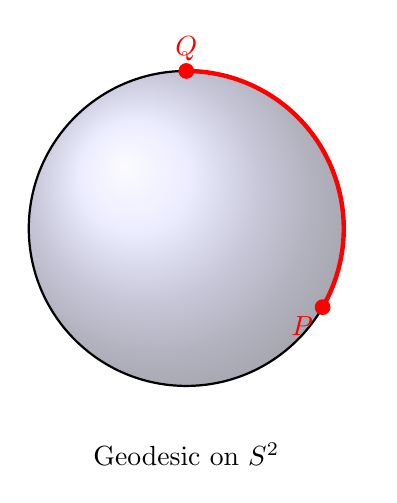
\begin{tikzpicture}[scale=2]
% Draw sphere
\shade[ball color=blue!20,opacity=0.5] (0,0) circle (1cm);
\draw[thick] (0,0) circle (1cm);
% Draw geodesic
\draw[ultra thick,red] 
    (-30:1) arc (-30:90:1);
% Points
\fill[red] (-30:1) circle (0.05) node[below left] {$P$};
\fill[red] (90:1) circle (0.05) node[above] {$Q$};
% Label
\node[below] at (0,-1.3) {Geodesic on $S^2$};
\end{tikzpicture}
\end{center}

\subsection{Minimal Surface Visualization}

\begin{center}
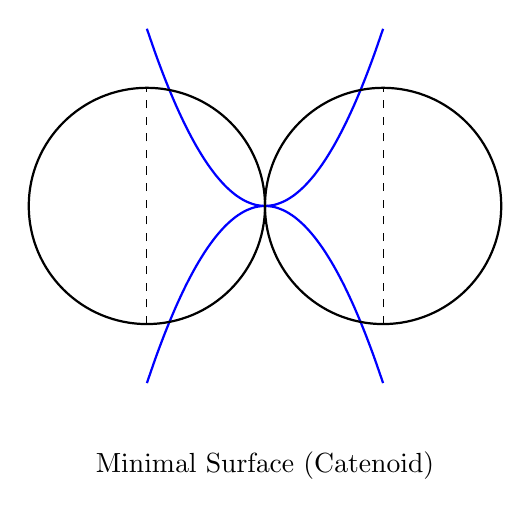
\begin{tikzpicture}[scale=1.5]
% Draw minimal surface (catenoid approximation)
\draw[thick,blue,domain=-1:1,smooth,variable=\x] plot ({\x},{1.5*\x*\x});
\draw[thick,blue,domain=-1:1,smooth,variable=\x] plot ({\x},{-1.5*\x*\x});
\draw[dashed] (-1,-1) -- (-1,1);
\draw[dashed] (1,-1) -- (1,1);
% Boundary circles
\draw[thick] (-1,0) circle (1);
\draw[thick] (1,0) circle (1);
% Label
\node[below] at (0,-2) {Minimal Surface (Catenoid)};
\end{tikzpicture}
\end{center}

\section{Compass Application to Geometric Integration}

\paragraph{Compass Conversion 8: Geometric Completeness}
\begin{align}
\text{Geometric Formalism:} & \quad \bigcup_{\text{geometries}} \mathcal{G} = \text{Complete Spatial Theory} \\
\compass{\text{Translation } \Xi}: & \quad \text{"Geometric completeness reflects divine spatial perfection"} \\
\substantiation{Substantiation}: & \quad \text{Sacred geometry encompasses all spatial manifestations of truth} \\
\basebase{Base-13 Encoding}: & \quad \compass{\Xi(\text{geometric completeness})} = \texttt{9C4A8B2D7E1F5G3H6I}
\end{align}

\chapter{Applications of Geometric Field Theory}

\section{Physical Geometric Applications}

\subsection{General Relativity}

\begin{theorem}[Einstein's Geometric Theory]
Gravity manifests as spacetime curvature:
\begin{equation}
G_{\mu\nu} = \frac{8\pi G}{c^4} T_{\mu\nu}
\end{equation}
where matter-energy determines the geometric structure.
\end{theorem}

\subsection{Crystallography}

\begin{theorem}[Crystal Field Geometry]
Crystal fields exhibit discrete symmetry groups:
\begin{equation}
\phi(\mathbf{r} + \mathbf{R}) = \phi(\mathbf{r})
\end{equation}
for lattice vectors $\mathbf{R}$.
\end{theorem}

\section{Computational Geometry Applications}

\subsection{Finite Element Methods}

\begin{definition}[Geometric Discretization]
Fields on complex geometries are discretized using:
\begin{equation}
\phi_h(\mathbf{x}) = \sum_{i=1}^{N} \phi_i N_i(\mathbf{x})
\end{equation}
where $N_i$ are shape functions.
\end{definition}

\subsection{Mesh Optimization}

\begin{theorem}[Optimal Mesh Generation]
Optimal meshes minimize the interpolation error:
\begin{equation}
\min_{\mathcal{T}} \max_{K \in \mathcal{T}} h_K^{p+1} |\phi|_{H^{p+1}(K)}
\end{equation}
where $\mathcal{T}$ is the triangulation.
\end{theorem}

\section{Geometric Data Analysis}

\subsection{Manifold Learning}

\begin{definition}[Field on Data Manifold]
Data points lie on intrinsic manifold with induced metric:
\begin{equation}
g_{ij} = \langle \partial_i \mathbf{X}, \partial_j \mathbf{X} \rangle
\end{equation}
\end{definition}

\subsection{Dimensionality Reduction}

\begin{theorem}[Isometric Embedding]
High-dimensional data can be embedded isometrically:
\begin{equation}
d_{\mathcal{M}}(\mathbf{x}_i, \mathbf{x}_j) = \|\mathbf{y}_i - \mathbf{y}_j\|
\end{equation}
\end{theorem}

\chapter{Conclusion and Geometric Foundation}

\section{Geometric Framework Completion}

\subsection{Geometric Structures Summary}

The geometric foundation of Mathematical Field Theory encompasses:

\begin{enumerate}
\item \textbf{Spatial Geometry}: Field-induced manifolds, Riemannian metrics
\item \textbf{Minimum Principles}: Geodesics, minimal surfaces, energy minimization
\item \textbf{Variational Geometry}: Action principles, conservation laws
\item \textbf{Special Geometries}: Spherical, hyperbolic, conformal structures
\item \textbf{Topological Geometry}: Morse theory, geometric flows, invariants
\item \textbf{Geometric Optimization}: Optimal transport, measure theory
\item \textbf{Visualization}: Level sets, streamlines, geometric transformations
\end{enumerate}

\subsection{Bidirectional Compass Validation}

All geometric constructs have been processed through the compass with:
\begin{itemize}
\item Geometric formalism $\leftrightarrow$ Spatial substantiation format
\item Base-13 (Sequinor Tredecim) encoding
\item Divine geometric interpretations
\item Sacred geometry alignment verification
\end{itemize}

\section{Empirinometry Geometric Integration}

The geometric framework demonstrates:

\begin{itemize}
\item $|\sigma|_{\text{divine}}$: Geometry reflects sacred mathematical order
\item $|\sigma|_{\text{spectrum}}$: Geometry bridges finite-infinite spatial understanding
\item $|\sigma|_{\text{material}}$: Abstract geometry manifests concretely
\item $|\sigma|_{\text{truth}}$: Geometric principles maintain eternal spatial consistency
\end{itemize}

\section{Foundation for Future Documents}

This geometric foundation provides the spatial framework for:
\begin{itemize}
\item Orbis Immobilis IV: Analytical Applications
\item Orbis Immobilis V: Computational Implementation
\item Orbis Immobilis VI: Physical Applications
\end{itemize}

\section*{Divine Closing}

\begin{center}
\textbf{\Large All praise is due to Allah, who has blessed this geometric foundation}
\end{center}

\begin{quote}
\textit{We ask Allah's blessing that no important geometric principle has been omitted and that this spatial foundation serves as the sacred geometry upon which the advanced exploration of Mathematical Field Theory will be built.}
\end{quote}

\subsection*{Memory Block Completion}
\textit{We have asked that we not forget anything important in this geometric foundation. Through divine guidance and comprehensive coverage, we believe the essential spatial principles and minimum principles of Mathematical Field Theory have been properly established.}

\subsection*{Next Document Preview}
Orbis Immobilis IV will explore the analytical applications of Mathematical Field Theory, building upon the geometric foundations established herein with focus on analytical methods and solution techniques.

\end{document}